\documentclass[tikz,border=0]{standalone}

\usepackage{tikz}
\usepackage{xcolor}

\begin{document}

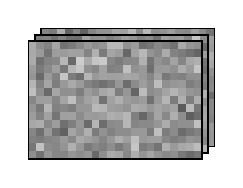
\begin{tikzpicture}[x=0.1cm,y=0.1cm]

% ============================================================
% 参数区（你只需要改这里）
% ============================================================

\def\Layers{8}      % 叠加层数：5~8 合理
\def\Alpha{0.2}    % 每层透明度
\def\Shift{0}    % 每层的空间偏移
\def\Cell{1}        % 单元格大小

% ============================================================
% 第一块区域
% ============================================================

\fill[fill=white] (0,0) rectangle (22,15);

\foreach \k in {1,...,\Layers} {
  \foreach \i in {0,...,21} {
    \foreach \j in {0,...,14} {

      % 随机灰度值（0~1）
      \pgfmathsetmacro{\g}{rnd}

      % 使用 inline RGB（灰度：R=G=B）
      \fill[
        fill={rgb,1:red,\g; green,\g; blue,\g},
        opacity=\Alpha
      ]
      (\i+\k*\Shift,\j+\k*\Shift) rectangle ++(\Cell,\Cell);
    }
  }
}

\draw[line width=0.6pt] (0,0) rectangle (22,15);

% ============================================================
% 第二块区域（偏移一圈）
% ============================================================

\fill[fill=white] (-0.8,-0.8) rectangle (21.2,14.2);

\foreach \k in {1,...,\Layers} {
  \foreach \i in {-0.8,...,20.2} {
    \foreach \j in {-0.8,...,13.2} {

      \pgfmathsetmacro{\g}{rnd}

      \fill[
        fill={rgb,1:red,\g; green,\g; blue,\g},
        opacity=\Alpha
      ]
      (\i+\k*\Shift,\j+\k*\Shift) rectangle ++(\Cell,\Cell);
    }
  }
}

\draw[line width=0.6pt] (-0.8,-0.8) rectangle (21.2,14.2);

% ============================================================
% 第三块区域（再偏移一圈）
% ============================================================

\fill[fill=white] (-1.6,-1.6) rectangle (20.4,13.4);

\foreach \k in {1,...,\Layers} {
  \foreach \i in {-1.6,...,19.4} {
    \foreach \j in {-1.6,...,12.4} {

      \pgfmathsetmacro{\g}{rnd}

      \fill[
        fill={rgb,1:red,\g; green,\g; blue,\g},
        opacity=\Alpha
      ]
      (\i+\k*\Shift,\j+\k*\Shift) rectangle ++(\Cell,\Cell);
    }
  }
}

\draw[line width=0.6pt] (-1.6,-1.6) rectangle (20.4,13.4);

\end{tikzpicture}

\end{document}
